\documentclass{article}

\usepackage{amsmath, amsthm, amssymb, amsfonts}
\usepackage{thmtools}
\usepackage{graphicx}
\usepackage{setspace}
\usepackage{geometry}
\usepackage{float}
\usepackage{hyperref}
\usepackage[utf8]{inputenc}
\usepackage[english]{babel}
\usepackage{framed}
\usepackage[dvipsnames]{xcolor}
\usepackage{tcolorbox}
\usepackage{diagbox}
\usepackage{amssymb}
\usepackage{enumerate}


\colorlet{LightGray}{White!90!Periwinkle}
\colorlet{LightOrange}{Orange!15}
\colorlet{LightGreen}{Green!15}

\newcommand{\HRule}[1]{\rule{\linewidth}{#1}}

\declaretheoremstyle[name=Ejemplo,]{thmsty}
\declaretheorem[style=thmsty,numberwithin=section]{theorem}
\tcolorboxenvironment{theorem}{colback=LightGray}

\declaretheoremstyle[name=Proposition,]{prosty}
\declaretheorem[style=prosty,numberlike=theorem]{proposition}
\tcolorboxenvironment{proposition}{colback=LightOrange}

\declaretheoremstyle[name=Principle,]{prcpsty}
\declaretheorem[style=prcpsty,numberlike=theorem]{principle}
\tcolorboxenvironment{principle}{colback=LightGreen}

\setstretch{1.2}
\geometry{
    textheight=9in,
    textwidth=5.5in,
    top=1in,
    headheight=12pt,
    headsep=25pt,
    footskip=30pt
}

% ------------------------------------------------------------------------------

\begin{document}

% ------------------------------------------------------------------------------
% Cover Page and ToC
% ------------------------------------------------------------------------------

\title{ \normalsize \textsc{}
		\\ [2.0cm]
		\HRule{1.5pt} \\
		\LARGE \textbf{\uppercase{Apuntes Probabilidad}
		\HRule{2.0pt} \\ [0.6cm] \LARGE{Tema 2: Vectores Aleatorios} \\
        {\large Doble Grado en Informática y Estadística (INdat)} \\
        \vspace*{10\baselineskip}}
		}

\author{\textbf{Autor} \\ 
		Juan Horrillo Crespo \\
		Universidad de Valladolid}

\maketitle

\newpage

\tableofcontents

\newpage

% ------------------------------------------------------------------------------


\section{Distribución conjunta de un vector aleatorio}


\subsection{Modelos para vectores aleatorios}

Cuando estudiamos experimentos aleatorios podemos tener interes en la variación conjunta de dos o más características o variables aleatorias del mismo. \\
Estas agrupaciones de varias características se conocen como vectores aleatorios. 
Por tanto el conjunto de vectores aleatorios posibles será ahora un subconjunto de 
\(\mathbb{R}^n\), siendo n la dimensión del vector aleatorio, osea el número de caracteristicas 
estudiadas. \\
Ademas de distribuciones discretas, continuas y mixtas, es posible encontrar algunas que no entre en ninguno
de los anteriores grupos, pero nuestro estudio se centrará en las distribuciones discretas y continuas. \\ \\

Llamaremos \textit{distribución conjunta del vector} al modelo probabilistico asociado a un vector aleatorio.
Un vector aleatorio se describe como \(X = (X_1, ... , X_n)\) siendo el resultado de la consideración conjunta de variables aleatorioas. 
Llamaremos \textit{distribución marginal} \(X_i\) a la distribución asociada a la caracteristica descrita por dicha variable por separado. \\
Es posible crear un vector mediante otros vectores de la forma \(X = (X_a, X_b)\); en estos casos, para referirnos a la distribución de \(X_a\) tambíen hablatemos de la \textit{Distribución marginal} de \(X_a\).

\subsection{Vectores aleatorios discretos}

Los modelos multivariantes discretos (modelos para vectores aleatorios) reproducen las
características de los modelos univariantes: \\
El conjunto de los valores posibles de \(X = (X_1,...,X_n)\) es un conjunto discreto
de elementos de \(\mathbb{R}^n\) y la probabilidad se concentra en esos elementos. Los
sucesos no elementales se calculan mediante las sumas de los elementales. \\
Emplearemos la notación \(X_1 = x_1, ...,  X_n = x_n\) para referirnos al suceso 
consistente en el que el vector aleatorio \(X = (X_1, ...,X_n)\) toma el valor 
\(x = (x_1, ..., x_n)\). De forma analoga, \((X_1 \in A_1, ..., X_n \in A_n)\) denota
el suceso consistente en que el valor de \(X\) es un elemento de \(A_1 \times ... \times A_n\). Es inmediato entonces
\[(X_1 \in A_1, ..., X_n \in A_n) = (X_1 \in A_1) \cap ... \cap (X_n \in A_n)\] \\
\\
A la función 
\[p(x_1, ..., x_n) = P(X_1 = x_1, ..., X_n = x_n), \qquad (x_1, ..., x_n) \in \mathbb{R}^n\]
la llamaremos \textit{función de masa de probabilidad conjunta} del vector \(X\).

\newpage

Con esta notación los modelos probabilísticos para vectores aleatorios discretos pueden
resumirse de la siguiente forma: \\ \\
\(X = (X_1, ..., X_n), \quad \Omega = \{ x^1, x^2, ..., x^i, ... \}, \quad x^i = (x^i_1, ..., x^i_n) \in \mathbb{R}^n\) \\
\(P(X_1 = x_1, ..., X_n = x_n) = p(x_1, ..., x_n);\) \\
\(p(x_1, ..., x_n) \geq 0, \quad \displaystyle\sum_{(x_1, ..., x_n) \in \Omega} p(x_1, ..., x_n) = 1\) \\ \\
\[P((X_1, ..., X_n) \in A) = P\left( \displaystyle\bigcup_{(x_1, ..., x_m) \in A} (X_1 = x_1, ..., X_n = x_n) \right) = \displaystyle\sum_{(x_1, ..., x_n) \in A} p(x_1, ..., x_n)\] \\

\subsection{Distribución conjunta de un vector aleatorio bidimensional}

Dadas \(X\) e \(Y\) dos variables aleatorias definidas sobre el mismo espacio muestral
\(\Omega\), la \qquad aplicación \((X,Y):\Omega \to \mathbb{R}^2\) es un vector
aleatorio bidimensional. \\
La distribución que describe simultáneamente el comportamiento de \(X\) e \(Y\) se 
llama \textit{distribución de probabilidad conjunta}. \\ \\
Dado un vector aleatorio \((X, Y)\) y dados \(x,y \in \mathbb{R}\), la \textit{función
de distribución conjunta} de \((X, Y)\) evaluada en \((x, y)\) se define como:
\[F_{X, Y}(x, y) = P(X \leq x, Y \leq y) = P((X \leq x) \cap (Y \leq y))\]
Esta función es útil principalmente en los casos continuos y mixtos.

\subsection{Vectores aleatorios discretos}

Dadas \(X\) e \(Y\) dos variables aleatorias discretas, el vector \((X, Y)\) será 
discreto y tiene \textit{función de probabilidad conjunta} 
\[p(x, y) = P(X = x, Y = y)\] \\
Por tanto tenemos las siguientes propiedades
\begin{enumerate}
    \item \(p(x, y) \geq 0\)
    \item \(\sum_{x}\sum_{y} p(x, y) = 1\)
\end{enumerate}
y una \textit{función de distribución conjunta}
\[F(x_{0}, y_{0}) = P(X \leq x_0, Y \leq y_0) = \sum_{x \leq x_0} \sum_{y \leq y_0} p(x, y)\]

\newpage

\begin{theorem}
    Consideremos el experimento aleatorio consistente en seleccionar al azar y sin reemplazamiento dos números del conjunto \(\{1, 2, 3, 4, 5, 6, 7, 8 \}\). Centremos nuestra atención en el vector aleatorio \((X, Y)\) en el que \(X\) es el mayor número elegido e \(Y\) es el menor. 
    Los posibles valores de \((X, Y)\) son los pares de números enteros \((i, j)\) que verifican \(1 \leq j < i \leq 8\). Si \((i, j)\) verifica esas condiciones entonces
    \[P(X = i, Y = j) = \frac{1}{\binom{8}{2}} = \frac{1}{28}\]
    (el experimento consiste, esencialmente, en escoger una subpoblación de tamaño 2 de una población con 8 elementos). \\
    A menudo es conveniente recoger en una tabla de doble entrada la función de masa de probabilidad de un vector aleatorio bidimensional. La tabla correspondiente a este ejemplo es la siguiente:
    \begin{center}
    \begin{tabular}{|l|ccccccc|}
    \hline
    \diagbox{X}{Y} & 1 & 2 & 3 & 4 & 5 & 6 & 7 \\
        \hline
        2 & \(\frac{1}{28}\) & 0 & 0 & 0 & 0 & 0 & 0 \\
        3 & \(\frac{1}{28}\) & \(\frac{1}{28}\) & 0 & 0 & 0 & 0 & 0 \\
        4 & \(\frac{1}{28}\) & \(\frac{1}{28}\) & \(\frac{1}{28}\) & 0 & 0 & 0 & 0 \\
        5 & \(\frac{1}{28}\) & \(\frac{1}{28}\) & \(\frac{1}{28}\) & \(\frac{1}{28}\) & 0 & 0 & 0 \\
        6 & \(\frac{1}{28}\) & \(\frac{1}{28}\) & \(\frac{1}{28}\) & \(\frac{1}{28}\) & \(\frac{1}{28}\) & 0 & 0 \\
        7 & \(\frac{1}{28}\) & \(\frac{1}{28}\) & \(\frac{1}{28}\) & \(\frac{1}{28}\) & \(\frac{1}{28}\) & \(\frac{1}{28}\) & 0 \\
        7 & \(\frac{1}{28}\) & \(\frac{1}{28}\) & \(\frac{1}{28}\) & \(\frac{1}{28}\) & \(\frac{1}{28}\) & \(\frac{1}{28}\) & \(\frac{1}{28}\) \\
        \hline
    \end{tabular} 
    \end{center}
    A partir de la función masa podemos calcular la probabilidad de cualquier otro suceso relacionado con \((X, Y)\). Por ejemplo, si \(A\) es el suceso "la diferencia entre los dos números elegidos es menor que 5", entonces
    \[P((X, Y) \in A) = P(X - Y < 5) = \displaystyle\sum_{(i, j)\in A}p(i, j)\]
    es decir, que \(P(X - Y < 5\) se calcula sumando los valores de la función de masa de probabilidad sombreados en la siguiente tabla
    \begin{center}
    \begin{tabular}{|l|ccccccc|}
    \hline
    \diagbox{X}{Y} & 1 & 2 & 3 & 4 & 5 & 6 & 7 \\
        \hline
        2 & \colorbox{gray}{\textcolor{white}{\(\frac{1}{28}\)}} & 0 & 0 & 0 & 0 & 0 & 0 \\
        3 & \colorbox{gray}{\textcolor{white}{\(\frac{1}{28}\)}} & \colorbox{gray}{\textcolor{white}{\(\frac{1}{28}\)}} & 0 & 0 & 0 & 0 & 0 \\
        4 & \colorbox{gray}{\textcolor{white}{\(\frac{1}{28}\)}} & \colorbox{gray}{\textcolor{white}{\(\frac{1}{28}\)}} & \colorbox{gray}{\textcolor{white}{\(\frac{1}{28}\)}} & 0 & 0 & 0 & 0 \\
        5 & \colorbox{gray}{\textcolor{white}{\(\frac{1}{28}\)}} & \colorbox{gray}{\textcolor{white}{\(\frac{1}{28}\)}} & \colorbox{gray}{\textcolor{white}{\(\frac{1}{28}\)}} & \colorbox{gray}{\textcolor{white}{\(\frac{1}{28}\)}} & 0 & 0 & 0 \\
        6 & \(\frac{1}{28}\) & \colorbox{gray}{\textcolor{white}{\(\frac{1}{28}\)}} & \colorbox{gray}{\textcolor{white}{\(\frac{1}{28}\)}} & \colorbox{gray}{\textcolor{white}{\(\frac{1}{28}\)}} & \colorbox{gray}{\textcolor{white}{\(\frac{1}{28}\)}} & 0 & 0 \\
        7 & \(\frac{1}{28}\) & \(\frac{1}{28}\) & \colorbox{gray}{\textcolor{white}{\(\frac{1}{28}\)}} & \colorbox{gray}{\textcolor{white}{\(\frac{1}{28}\)}} & \colorbox{gray}{\textcolor{white}{\(\frac{1}{28}\)}} & \colorbox{gray}{\textcolor{white}{\(\frac{1}{28}\)}} & 0 \\
        7 & \(\frac{1}{28}\) & \(\frac{1}{28}\) & \(\frac{1}{28}\) & \colorbox{gray}{\textcolor{white}{\(\frac{1}{28}\)}} & \colorbox{gray}{\textcolor{white}{\(\frac{1}{28}\)}} & \colorbox{gray}{\textcolor{white}{\(\frac{1}{28}\)}} & \colorbox{gray}{\textcolor{white}{\(\frac{1}{28}\)}} \\
        \hline
    \end{tabular} 
    \end{center}
    Por lo tanto \(P(X - Y < 5) = \frac{22}{28} \approx 0,7857\)
\end{theorem}

\subsection{Vectores aleatorios continuos}

Diremos que el vector aleatorio \(X = (X_1, ..., X_n)\) es continuo y con 
función de densidad \(f(x_1, ..., x_n)\) si las probabilidades de los
sucesos de interés dentro del modelo se calculan segun la regla
\[P(X \in A) = \int_A f(x_1, ..., x_n)dx_1 \dotsi dx_n\]
Para que la anterior expresión defina un modelo probabilistico correcto
la función \(f\) debe verificar las siguientes condiciones
\begin{enumerate}
    \item \(f(x_1, ..., x_n) \geq 0, \qquad (x_1, ..., x_n) \in \Omega \subset \mathbb{R}^n\)
    \item \(\int_\Omega f(x_1, ..., x_n) dx_1 \dotsi dx_n = 1\)
\end{enumerate}
donde \(\Omega\), el conjunto de valores posibles de \(X\), es subconjunto
de \(\mathbb{R}^n\).
\subsubsection{Vector aleatorio continuo bidimensional}
Dados \(X\) e \(Y\) dos variables aleatorias continuas, el vector 
aleatorio \((X, Y)\) será contiuo y tiene \textit{función de densidad 
conjunta} \(f(x, y)\) que satisface
\begin{enumerate}
    \item \(f(x, y) \geq 0;\)
    \item \(\int\int f(x, y)dx dy = 1\)
\end{enumerate}
y una \textit{función de distribución conjunta} descrita como
\[F(x_0, y_0) ) P(X \leq x_0, Y \leq y_0) =  \int_{-\infty}^{x_0}\int_{-\infty}^{y_0} f(x, y)dy dx\]
Para calcular la probabilidad de que un suceso esté entre dos valores \((a, c)\) y \((b, d)\) tenemos que
\[P(a \leq X \leq b, c \leq Y \leq d) = \int_{a}^{b}\int_{c}^{d}f(x, y)dydx\]
\[F(x, y) = \int_{-\infty}^{x}\int_{-\infty}^{y} f(x, y)dydx\]
y ademas
\[f(x, y) = \frac{\delta^2}{\delta x\delta y}F(x, y)\]

\newpage

Aquí se pueden ver algunos ejemplos de funciones de densidad variables. El
analisis de la probabilidad consiste en calcular el volumen encerrado
bajo la superficie.
\vspace*{\fill}
	\begin{figure}[htbp]
        \center
        \includegraphics[scale=0.8]{img/FunciónDensidadBivariable.png}
        \caption{Una función de densidad bivariable}
    \end{figure}
\vspace*{\fill}
\vspace*{\fill}
    \begin{figure}[htbp]
        \center
        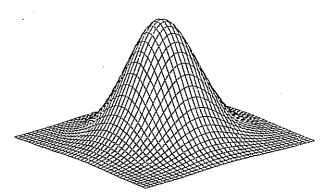
\includegraphics[scale=1]{img/NormalBivariable.png}
        \caption{Densidad normal bivariable}
    \end{figure}
\vspace*{\fill}

\newpage

\begin{theorem}
    Consideremos el experimento consistente en seleccionar un punto al azar en un círculo de radio unidad 
    (suponemos centrado en \((0, 0)\)). Llamaremos \(X\) e \(Y\) a la abcisa y a la ordenada del punto elegido. 
    La elección puramente al azar se puede modelizar con al función de densidad
    
    \[f(x, y) = \left\{
        \begin{array}{rcr}
            \frac{1}{\pi}   & si    & x^2 + y^2 \leq 1 \\
            0               & si    & x^2 + y^2 > 1
        \end{array}
    \right\}\]

    Esta función es una función de densidad. Fácilmente comprobamos que su integral es uno:

    \[\int_{\{(x, y) \big{/} x^2 + y^2 \leq 1\}} f(x, y)dxdy = \int_{-1}^{1} \left(\int_{-\sqrt{1 - x^2}}^{\sqrt{1 - x^2}} \frac{1}{\pi}dy\right)dx =\]
    \[=\frac{1}{\pi}\int_{-1}^{1} 2\sqrt{1 - x^2}dx = \frac{\pi}{\pi} = 1\]

    El cálculo de probabilidades dentro de este modelo se efectúa integrando la función de densidad en la región adecuada. 
    Consideremos los sucesos $A$ = \textit{"el punto elegido dista del origen menos de 0.5 unidades"} y $B$ = \textit{"la abcisa del 
    punto elegido está dentro del intervalo $(0.3, 0.8)$"}.
    
    \[P((X, Y) \in A) = P(X^2 + Y^2 < 0.5^2) = \int_{\{(x, y) \big{/} x^2 + y^2 < 0.25\}} f(x, y)dxdy =\]
    \[= \int_{-0.5}^{0.5} \left(\int_{-\sqrt{0.25 - x^2}}^{\sqrt{0.25 - x^2}} \frac{1}{\pi}dy\right)dx = \frac{1}{\pi}\int_{-0.5}^{0.5} 2\sqrt{0.25 - x^2}dx = \frac{\pi}{4\pi} = 0.25\]

    \[ P((X, Y) \in B) = P(0.3 < X < 0.8) = \int_{\{ (x, y) \big{/} 0.3 < x < 0.8 \}} f(x, y)dxdy = \]
    \[ = \int_{0.3}^{0.8} \left( \int_{-\sqrt{1 - x^2}}^{\sqrt{1 - x^2}} \frac{1}{\pi}dy \right) dx = \frac{1}{\pi} \int_{0.3}^{0.8} 2\sqrt{1 - x^2} dx = \]
    \[ \frac{1}{\pi} \left[ \arcsin x + x\sqrt{1 - x^2} \right]_{x = 0.3}^{x = 0.8} \approx 0.2599 \]

\end{theorem}

\begin{figure}[htbp]
    \center
    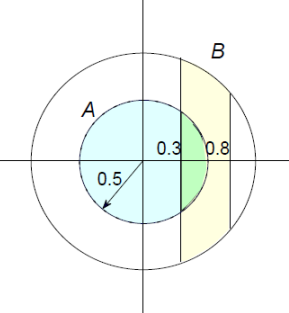
\includegraphics[scale=0.6]{img/Ejemplo2.png}
    \caption{Circunferencia de radio unidad y los conjuntos A y B}
\end{figure}


\section{Distribuciones marginales y condicionadas}


\subsection{Distribuciones marginales}

A la distrubución de cada variable de las que componen un vector aleatorio se le denomina \textit{distribución marginal}.
Dado el vector aleatorio $(X, Y)$ podemos hablar de la \textit{distribución marginal de $X$} y de la \textit{distribución marginal de $Y$}. \\
\subsubsection{Variables discretas} 
Dadas $X$ e $Y$ variables discretas con función de probabilidad conjunta $p(x, y)$, las funciones de probabilidad 
marginales de ambas variables son:

\[ p_{X}(x) = P(X = x) = \sum_{y}P(X = x, Y = y) = \sum_{y}p(x, y) \]
\[ p_{Y}(y) = P(Y = y) = \sum_{y}P(X = x, Y = y) = \sum_{x}p(x, y) \] 

\begin{theorem}
    Podemos obtener la distribución marginal de $X$ a partir de la tabla con la función de masa de probabilidad 
    conjunta sumando los valores por filas. Análogamente, sumando los valores de las columnas obtendremos la de $Y$:

    \begin{center}
        \begin{tabular}{|l|ccccccc|c|}
        \hline
        \diagbox{X}{Y} & 1 & 2 & 3 & 4 & 5 & 6 & 7 & $P_{X}$\\
            \hline
            2 & \(\frac{1}{28}\) & 0 & 0 & 0 & 0 & 0 & 0 & \(\frac{1}{28}\) \\
            3 & \(\frac{1}{28}\) & \(\frac{1}{28}\) & 0 & 0 & 0 & 0 & 0 & \(\frac{2}{28}\) \\
            4 & \(\frac{1}{28}\) & \(\frac{1}{28}\) & \(\frac{1}{28}\) & 0 & 0 & 0 & 0 & \(\frac{3}{28}\) \\
            5 & \(\frac{1}{28}\) & \(\frac{1}{28}\) & \(\frac{1}{28}\) & \(\frac{1}{28}\) & 0 & 0 & 0 & \(\frac{4}{28}\) \\
            6 & \(\frac{1}{28}\) & \(\frac{1}{28}\) & \(\frac{1}{28}\) & \(\frac{1}{28}\) & \(\frac{1}{28}\) & 0 & 0 & \(\frac{5}{28}\) \\
            7 & \(\frac{1}{28}\) & \(\frac{1}{28}\) & \(\frac{1}{28}\) & \(\frac{1}{28}\) & \(\frac{1}{28}\) & \(\frac{1}{28}\) & 0 & \(\frac{6}{28}\) \\
            7 & \(\frac{1}{28}\) & \(\frac{1}{28}\) & \(\frac{1}{28}\) & \(\frac{1}{28}\) & \(\frac{1}{28}\) & \(\frac{1}{28}\) & \(\frac{1}{28}\) & \(\frac{7}{28}\) \\
            \hline
            $P_{Y}$ & \(\frac{7}{28}\) & \(\frac{6}{28}\) & \(\frac{5}{28}\) & \(\frac{4}{28}\) & \(\frac{3}{28}\) & \(\frac{2}{28}\) & \(\frac{1}{28}\) & \\
            \hline
        \end{tabular}     
    \end{center}

        Por tanto

        \[ P(X = 3) = p_{X}(3) = \frac{3}{28} \]

        \[ P(Y = 2) = p_{Y}(2) = \frac{6}{28} \]

\end{theorem}

\newpage

\subsection{Variables continuas}
Dadas $X$ e $Y$ variables continuas con función de densidad conjunta $f(x, y)$, las funciones de densidad marginales
de ambas variables son

\[ f_{X}(x) = \int_{-\infty}^{\infty} f(x, y)dy \]
\[ f_{Y}(y) = \int_{-\infty}^{\infty} f(x, y)dx \]

\begin{theorem}
    Continuando con el vector $(X, Y)$ del ejemplo continuo anterior cuya densidad conjunta uniforme sobre el 
    círculo unidad era

    \[f(x, y) = \left\{
        \begin{array}{rcr}
            \frac{1}{\pi}   & si    & x^2 + y^2 \leq 1 \\
            0               & si    & x^2 + y^2 > 1
        \end{array}
    \right\}\]

    La densidad marginal para $X$ es:

    \[ f_{X}(x) = \int_{-\sqrt{1 - x^2}}^{\sqrt{1 - x^2}} f(x, y) dy = \int_{-\sqrt{1 - x^2}}^{\sqrt{1 - x^2}} \frac{dy}{\pi} = \frac{2}{\pi} \sqrt{1 - x^2}, \quad -1 < x < 1 \]

\end{theorem}

\subsection{Distribuciones condicionadas}

La idea de una probabilidad condicionada se puede incorporar a los modelos de vectores aleatorios. Supongamos que el experimento
de interés se recoge en el vector aleatorio $X = (X_a, X_b)$ del que sabemos que el subvector $X_a$ toma el valor $x_a$. \\
El grado de creencia en los sucesos relativos a la otra parte del experimento, $X_b$, se verá modificado. A la distribución de $X_b$
modificada para incorporar esta información la llamaremos \textit{distribución de $X_b$ condicionada a $X_a$}.
En esta sección se estudiará la manera en la que se actualiza la distrubución de un vector aleatorio en estas circunstancias, 
considerando por separado los casos discreto y continuo. 
\subsubsection{Caso discreto}
Las distribuciones condicionadas se obtienen a partir de la definición de probabilidad condicionada
de sucesos. Supongamos por ejemplo que ha ocurrido ($X_a$ = $x_a$). La probabilidad de que ($X_b$ = $x_b$)
será
\[ P\left( {X_{b} = x_{b}} \bigg{/} {X_{a} = x_{a}} \right) = \frac{P(X_{a} = x_{a}, X_{b} = x_{b})}{P(X_{a} = x_{a})} = \frac{p(x_{a}, x_{b})}{p_{x_{a}}(x_{a})} \]

A la función de masa de probabilidad que incorpora la información ($X_a$ = $x_a$) se le llama \textit{función de masa de probabilidad condicionada por $x_a$}
y se denota $p(x_b|x_a)$, es decir 

\[ p\left( {x_b} \bigg{/} {x_a} \right) = P\left( {X_{b} = x_{b}} \bigg{/} {X_{a} = x_{a}} \right) \]

\newpage

Esta función está bien definida para 

\[ P(X_{a} = x_{a}) > 0 \qquad p\left(x_b \bigg{/} x_a\right) = \frac{p(x_a, x_b)}{p_{x_{a}}(x_a)} \]

Esta última igualdad reescrita de la forma siguiente

\[ p(x_a, x_b) =  p_{x_a}(x_a)p\left( x_b \bigg{/} x_a \right)\]

o, equivalente, en la forma

\[ P(X_a = x_a, X_b = x_b) = P(X_a = x_a)P\left( X_b = x_b \bigg{/} X_a = x_a \right) \]

se conoce como \textit{``Regla de la multiplicación''}. Esta regla nos permite obtener la distribución conjunta
a partir de las distribuciones marginales y condicionadas.

\begin{theorem}
    
    Se lanza un dado. Lllamaremos $X$ al resultado obtenido. A continuación se lanzan $X$ monedas. Representaremos por $Y$
    el número de caras obtenidas. Calcula la distribución de $X$, la distribución de $Y$ condicionada por $X$, la distribución
    conjunta de $(X, Y)$ y la distribución marginal de $Y$. \\
    Obviamente la dsitribución de $X$ es $P(X = i) = \frac{1}{6},\quad i = 1,2,\dots, 6$. Si se lanzan $i$ monedas, el número
    de resultados diferentes que podemos obtener es $2^{i}$ (Combinatoria de $i$ elementos tomados de $2$ en $2$). \\
    De esas $2^{i}$ posibilidades, en $\binom{i}{j}$ se registran $j$ caras. Asumiendo que las monedas no estan sesgadas
    podemos aplicar la \textit{Regla de Laplace} para obtener

    \[ P\left( Y = j \bigg{/} X = i \right) = \binom{i}{j}\frac{1}{2^{i}} \]

    para $0 \leq j \leq i$. La distribución conjunta es, por tanto,

    \[ P(X = i, Y = j) = P(X = i) P\left( Y = j \bigg{/} X = i \right) = \frac{1}{6}\binom{i}{j}\frac{1}{2^{i}} \]

    para $i = 1,2,\dots,6$ y $0 \leq j \leq i$. Podemos expresar la distribución conjunta en la siguiente tabla:

    \begin{center}
        \begin{tabular}{l|ccccccc}
        \diagbox{X}{Y} & 0 & 1 & 2 & 3 & 4 & 5 & 6\\
            \hline
            1 & \(\frac{1}{6}\frac{1}{2}\) & \(\frac{1}{6}\frac{1}{2}\) & 0 & 0 & 0 & 0 & 0 \\
            2 & \(\frac{1}{6}\frac{1}{4}\) & \(\frac{1}{6}\frac{5}{4}\) & \(\frac{1}{6}\frac{1}{4}\) & 0 & 0 & 0 & 0 \\
            3 & \(\frac{1}{6}\frac{1}{8}\) & \(\frac{1}{6}\frac{3}{8}\) & \(\frac{1}{6}\frac{3}{8}\) & \(\frac{1}{6}\frac{1}{8}\) & 0 & 0 & 0 \\
            4 & \(\frac{1}{6}\frac{1}{16}\) & \(\frac{1}{6}\frac{4}{16}\) & \(\frac{1}{6}\frac{6}{16}\) & \(\frac{1}{6}\frac{4}{16}\) & \(\frac{1}{6}\frac{1}{16}\) & 0 & 0 \\
            5 & \(\frac{1}{6}\frac{1}{32}\) & \(\frac{1}{6}\frac{5}{32}\) & \(\frac{1}{6}\frac{10}{32}\) & \(\frac{1}{6}\frac{10}{32}\) & \(\frac{1}{6}\frac{5}{32}\) & \(\frac{1}{6}\frac{1}{32}\) & 0 \\
            6 & \(\frac{1}{6}\frac{1}{64}\) & \(\frac{1}{6}\frac{6}{64}\) & \(\frac{1}{6}\frac{15}{64}\) & \(\frac{1}{6}\frac{20}{64}\) & \(\frac{1}{6}\frac{15}{64}\) & \(\frac{1}{6}\frac{6}{64}\) & \(\frac{1}{6}\frac{1}{64}\) \\
            \hline
            $P(Y)$ & $0.1641$ & $0.3125$ & $0.2578$ & $0.1667$ & $0.0755$ & $0.0208$ & $0.0026$ \\
        \end{tabular}
    \end{center}

    Sumando por columnas obtendremos la distribución marginal de Y, recogida en el margen inferior de la tabla


\end{theorem}

\subsubsection{Caso continuo}
En el caso continuo la distribución condicionada es también continua. A la función de densidad correspondiente se le llama función
de densidad condicionada y se denota mediante cualquiera de los dos simbolos siguientes:

\[ f\left( x_a \bigg{/} x_b \right) \quad \text{o} \quad f_{X_b / X_a = x_a}(x_b) \]

Cualquiera de los dos representa la densidad el vector aleatorio $X_b$ cuando se incorpora al modelo de información consistente en
que $X_a$ toma el valor $x_a$. \\
Se puede comprobar que la densidad condicionada se calcula de forma análoga a la función de densidad condicionada del caso discreto:

\[ f\left( x_a \bigg{/} x_b \right) = \frac{f(x_a, x_b)}{f_{X_a}}(x_a) \]

es decir, que la densidad condicionada se obtiene dividiendo la densidad conjunta por la densidad marginal de la variable (o vector)
por la que condicionamos. \\
Igual que en el caso discreto, reescribir convenientemente la igualdad anterior nos conduce a una nueva \textit{``Regla de la multiplicación''}:

\[ f(x_a, x_b) = f_{X_a}(x_a)f\left( x_a \bigg{/} x_b \right) \]

\begin{theorem}
    
    Consideremos el experimento aleatorio consistente en elegir un punto al azar, $x$, en el intervalo $(0, 1)$. Una vez elegido $x$ escogemos
    otro punto $y$ al azar en el intervalo $(0, x)$. Llamemos $(X, Y)$ al vector aleatorio cuyas coordenadas son los puntos elegidos por el 
    procedimiento anterior. Calcular
    \begin{enumerate}[a)]
        \item la densidad conjunta de $(X, Y)$
        \item la densidad marginal de $Y$
        \item la probabilidad de que $Y$ tome un valor menor que $0.8$
    \end{enumerate}

    // Falta la resolución de a)

    Teniendo $f(x, y) = \frac{1}{x}$ función de densidad conjunta, podemos calcular la densidad marginal de $Y$:

    \[ f_{Y}(y) = \int_{y}^{1}f(x, y)dx = \int_{y}^{1}\frac{1}{x}dx = -\log{y}, \quad 0 < y < 1 \]

    La función de distribución asociada a Y es

    \[ F_{Y}(y) = \int_{0}^{y}f_{y}(t)dt = y(1 - \log_{y}), \quad 0 < y < 1 \]

    La probabilidad que se pide en el apartado c) es fácil de calcular a partir de $F_{Y}$:

    \[ P(Y < 0.8) = F_{Y}(0.8) = 0.8(1 - \log{0.8}) \approx 0.9785 \]

\end{theorem}

\newpage


\section{Distribución multinomial}


Dado un experimento aleatorio con $k$ resultados posibles, de tal modo que la probabilidad de cada resultado $p_1, p_2, \dots, p_k$ se mantiene constante,
un vector aleatorio $(X_1, X_2, \dots, X_k)$ sigue distribución multinomial si cada $X_{i}$ representa el número de veces que ocurre el resultado $i$-esimo
en $n$ repeticiones independientes del experimento. \\
Dados $0 \leq x_1, x_2, \dots, x_k \leq n$ y $0 \leq p_1, p_2, \dots, p_k \leq 1$ con $\sum_{i = 1}^{k}x_i = n$ y $\sum_{i = 1}^{k}p_i = 1$, si 
$(X_1, X_2, \dots, X_k)$ sigue distribución multinomial, tenemos

\[ P(X_1 = x_1, X_2 = x_2,\dots,X_k = x_k) = \frac{n!}{x_{1}!x_{2}!\cdots x_{k}!}p_{1}^{x_1}p_{2}^{x_2}\cdots p_{k}^{x_k}\]

Propiedades:
\begin{itemize}
    \item Todas las distribuciones marginales de un vector multinomial son multinomiales (binomiales en su caso)
    \item Todas las distribuciones condicionales de un vector multinomial son multinomiales (binomiales en su caso)
\end{itemize}
Por ejemplo, podemos decir que, si $(X_1,\dots,X_k)\thicksim\mathcal{M}(n;p_1,\dots,p_k)$ entonces:
\begin{itemize}
    \item $X_i\thicksim b(n, p_i),\quad i = 1,\dots,k$
    \item $X_1 + \cdots + X_i\thicksim b(n, p_1 + \cdots + p_k), \quad i = 1, \dots, k$
\end{itemize}


\section{Vectores mixtos}


Sea $(X, Y)$ vector aleatorio tal que conocemos la distribución  de $Y$ condicionada a $X = x_0$ y la distribución de $X$, en los siguentes casos,
¿cómo podemos obtener la ley de $Y$?
\begin{itemize}
    \item $X$ e $y$ son v.a. discretas
    \item $X$ e $Y$ son v.a. continuas
    \item $X$ es discreta e $Y$ es continua
    \item $X$ es continua e $Y$ es discreta
\end{itemize}


\section{Independencia entre variables aleatorias}


Dos variable aleatorias $X$ e $Y$ se dicen \textit{independientes} si el conocimiento del valor que toma una, no nos aporta información sobre el valor 
que tomará la otra. \\
Para cualesquiera $A, B \subset \mathbb{R}$,

\[ P((X \in A) \cap (Y \in B)) = P(X \in A)P(Y \in B) \]

Equivalentemente, para cualesquiera $x, y \in \mathbb{R}$

\[ P((X \leq x) \cap (Y \leq y)) = P(X \leq x)P(Y \leq y) \]

\newpage

\textbf{Propiedad:} Si $X$ e $Y$ son independientes, entonces

\[ Var[X + Y] = Var[X] + Var[Y] \]

\begin{itemize}
    \item Variables aleatorias \textbf{discretas} son Indep. si
    \begin{enumerate}
        \item $p(y | x) = p_{Y}(y) \qquad \text{para cualesquiera $x, y$ o bien}$
        \item $p(x | y) = p_{X}(x) \qquad \text{para cualesquiera $x, y$ o bien}$
        \item $p(x, y) = p(x | y)p_{Y}(y) = p_{X}(x)p_{Y}(y) $
    \end{enumerate}
    \item Variables aleatorias \textbf{continuas} son Indep. si
    \begin{enumerate}
        \item $f(y | x) = f_{Y}(y) \qquad \text{para cualesquiera $x, y$ o bien}$
        \item $f(x | y) = f_{X}(x) \qquad \text{para cualesquiera $x, y$ o bien}$
        \item $f(x, y) = f(x | y)f_{Y}(y) = f_{X}(x)f_{Y}(y) $
    \end{enumerate}
\end{itemize}


\section{Características de un vector aleatorio}


\subsection{Esperanza}

El vector de medias de $X$ es el vector cuyas componentes son las esperanzas de cada componente de $X$

\[ E[X] = \left( \begin{matrix}
    E[X_1] \\
    E[X_2] \\
    \vdots \\
    E[X_n] 
\end{matrix} \right) \]

\subsection{Covarianza}

Cuando tenemos que estudiar la variación conjunta de dos variables aleatorias que forman un vector aleatorio,
la descripción individual de cada una de las variables por medio de los correspondientes parámetros poblacionales
resulta insuficiente como resumen numérico del vector aleatorio pues no informa de un aspecto tan importante
como es la asociación entre las dos variables. \\
Las versiones poblacionales de las medidas de asociación que se manejan en Estadística Descriptiva nos servirán
ahora para cuantificar la asociación entre variables aleatorias estudiadas sobre la misma población. \\

\textbf{Covarianza:} La covarianza de dos variables aleatorias $X$ e $Y$ se denota $Cov(X, Y)$ ó $\sigma_{X,Y}$
y se define como el valor medio de los productos cruzados de las distancias de los valores de cada una de las
variables respecto a su media, es decir

\[ Cov(X, Y) = \sigma_{X, Y} = E[(X - E[X])(Y - E[Y])] \]

\newpage

Para el \textit{Caso discreto} tenemos
\begin{itemize}
    \item $\Omega = \{(x_i, y_j)/ i, j = 1, 2, \dots\} \subset \mathbb{R}^2$
    \item f.m.p: $p(x_i, y_j)$
\end{itemize}

\[ \sigma_{X, Y} = \displaystyle\sum_{i,j}(x_i - \mu_{X})(y_j - \mu_{Y})p(x_i, y_j) \]

En cambio para el \textit{Caso continuo} tenemos
\begin{itemize}
    \item $\Omega = \subset \mathbb{R}^2$
    \item f.dens: $f(x, y)$
\end{itemize}

\[ \sigma_{X, Y} = \int (x - E[X])(y - E[Y])f(x, y)dx \]

Dada la definición de covarianza de un vector podemos realizar las siguientes observaciones:

\begin{itemize}
    \item La varianza indica el sentido de la asociación a través del signo:
    \begin{enumerate}
        \item $Cov(X, Y) > 0 \Rightarrow$ asociación lineal creciente
        \item $Cov(X, Y) < 0 \Rightarrow$ asociación lineal decreciente
        \item $Cov(X, Y) = 0 \Rightarrow$ indica la ausencia de asociación lineal. En particular, si $(X, Y)$ son variables aleatorias independientes
                se prueba facilmente que $E[XY] = E[X]E[Y]$, con lo que $Cov(X, Y) = 0$
    \end{enumerate}
    \item La covarianza es invariante por cambios de localización de las variables, pero no por cambios de escala:
     
    \[ (X, Y) \text{vector aleatorio,} \quad (X', Y') = (aX + b, cY + d), a, c > 0 \implies \]
    \[ \implies Cov(X', Y') = acCov(X, Y) \]

    \item La covarianza no se puede usar directamente como medida de asociación lineal porque su valor depende de las unidades de medida de las variables.
\end{itemize}

La covarianza tiene las siguientes \textbf{propiedades}:
\begin{itemize}
    \item $Cov(X, Y) = E[XY] - E[X]E[Y]$
    \item si $X$ e $Y$ son independientes, entonces $Cov(X, Y) = 0$
    \item $Cov(X, Y) = 0$ no garantiza que $X$ e $Y$ sean independientes
    \item $Cov(X, X) = Var(X)$
    \item $Cov(aX + b, cY + d) = acCov(X, Y),\quad a, c >0$
    \item $Cov(\sum_{i}X_i, \sum_{j}Y_j) = \sum_{i}\sum_{j}Cov(X_i, Y_j)$
    \item $Var(X + Y) = Var(X) + Var(Y) + 2Cov(X, Y)$
    \item $Var(\sum_{i}X_i) = \sum_{i}Var(X_i) + \sum_i\sum_kCov(X_i, X_k)$
\end{itemize}

\newpage

\subsection{Correlación}

El \textbf{Coeficiente de Correlación} es una medida de asociación lineal entre variables aleatorias que se define a partir de la covarianza
y evitando los inconvenientes de esta: 

\[ \rho(X, Y) = \rho_{X, Y} = \frac{Cov(X, Y)}{\sqrt{Var(X)Var(Y)}} = \frac{\sigma_{X, Y}}{\sigma_X\sigma_Y} \]

Dada la definición de correlación de un vector podemos realizar las siguientes observaciones: 

\begin{itemize}
    \item El coeficiente de correlación es invariante por cambios de locaclización y escala en las variables:
    
    \[ (X, Y) \text{vector aleatorio}, (X', Y') = (aX + b, cY + d), a, c > 0 \implies \]
    \[ \implies \rho(X', Y') = \rho(X, Y) \]

    \item El coeficiente de correlación es adimensional, no tiene unidades. De hecho, el coeficiente de correlación es igual a la covarianza
            de las variables tipificadas:

    \[ (X, Y) \text{vector aleatorio}, \quad Z_{X} = \frac{X - \mu_{X}}{\sigma_X}, Z_{Y} = \frac{Y - \mu_Y}{\sigma_Y} \implies \]
    \[ \implies \rho(X, Y) = Cov(Z_X, Z_Y) \]

    \item El valor del coeficiente de correlación está acotado:
    
    \[ |\rho(X, Y)| \leq 1 \]


\end{itemize}

La correlación tiene las siguientes \textbf{propiedades}:
\begin{itemize}
    \item Si $X$ e $Y$ son independientes, entonces $\rho(X, Y) = 0$
    \item $\rho(X, Y) = 0$ no garantiza que $X$ e $Y$ sean independientes
    \item $|\rho(X, Y)| \leq 1$
    \item Si $a, c > 0$, entonces $\rho(aX + b, cY + d) = \rho(X, Y)$
    \item $|\rho(X, X)| = 1$
    \item Si $a > 0$ entonces $|\rho(X, aX + b)| = 1$
\end{itemize}

\newpage

\subsection{Matriz de covarianzas}

La matriz de varianzas y covarianzas, o simplemente matriz de covarianzas, es simetrica y semidefinida positiva. Se define como

\[ \Sigma_{X} = \left( \begin{matrix}
        Var[X_1] & Cov(X_1, X_2) & \cdots & Cov(X_1, X_n) \\
        Cov(X_2, X_1) & Var[X_2] & \cdots & Cov(X_2, X_n) \\
        \vdots & \vdots & \ddots & \vdots \\
        Cov(X_n, X_1) & Cov(X_n, X_2) & \cdots & Var[X_n]
\end{matrix} \right) \]

\subsection{Matriz de correlaciones}

La matriz de correlaciones es simetrica y semidefinida positiva. Se define como

\[ R_{X} = \left( \begin{matrix}
        1 & \rho(X_1, X_2) & \cdots & \rho(X_1, X_n) \\
        \rho(X_2, X_1) & 1 & \cdots & \rho(X_2, X_n) \\
        \vdots & \vdots & \ddots & \vdots \\
        \rho(X_n, X_1) & \rho(X_n, X_2) & \cdots & 1
\end{matrix} \right) \]

\subsection{Características numéricas de la distribución multinomial}

\begin{itemize}
    \item Medias: $\mu_{X_i} = E[X_i] = np_i$
    \item Varianzas: $\sigma_{X_i}^2 = Var[X_i] = np_i(1 - p_i)$
    \item Covarianzas: $\sigma_{X_i, X_j} = Cov(X_i, X_j) = -np_ip_j$
\end{itemize}


\section{Transformaciones de vectores aleatorios}


Dado el vector aleatorio $X = (X_1, X_2, \dots, X_n)$ con función de densidad conjunta $f_X(x_1, x_2, \dots, x_n)$, lo tranformamos
en otro vector aleatorio $Y = (Y_1, Y_2, \dots, Y_n)$ con la misma dimensión

\[ \left( \begin{matrix}
    Y_1 = g_1(X_1,X_2,\dots,X_n) \\
    Y_2 = g_2(X_1,X_2,\dots,X_n) \\
    \vdots \\
    Y_n = g_n(X_1,X_2,\dots,X_n)
\end{matrix} \right) \]

de tal modo que existan transformadas inversas. La función de densidad continua será

\[ f_Y(y_1, y_2, \dots, y_n) = f_X(g^{-1}(y_1, y_2, \dots, y_n))|J| \quad \text{donde} \quad J = 
\left| \begin{matrix}
    \frac{dx_1}{dy_1} & \frac{dx_1}{dy_2} & \cdots & \frac{dx_1}{dy_n} \\
    \frac{dx_2}{dy_1} & \frac{dx_2}{dy_2} & \cdots & \frac{dx_2}{dy_n} \\
    \vdots & \vdots & \ddots & \vdots \\
    \frac{dx_n}{dy_1} & \frac{dx_n}{dy_2} & \cdots & \frac{dx_n}{dy_n}
\end{matrix} \right| \]


\newpage

\subsection{Convolución}

Si $X$ e $Y$ son variables aleatorias idependientes con funciones de densidad $f_X(x)$ y $f_Y(y)$, respectivamente, entonces la función de densidad de 
$Z = X + Y$ es

\[ f_Z(z) = \int_{-\infty}^{\infty}f_{X}(z - x)f_{Y}(x)dx \]

\subsection{Transformaciones lineales}

Dado $X$ un vector aleatorio $n$-dimensional y $u$ un vector en $\mathbb{R}^n$, la variable aleatoria $Y = u^tX$ cumple

\[ E[Y] = E[u^tX] = u^tE[X] \]
\[ Var[Y] = Var[u^tX] = u^t\Sigma_Xu \]

Dado $X$ un vector aleatorio $n$-dimensional y $A$ una matriz $m \times n$-dimensional, el vector aleatorio $Y = AX$($m$-dimensional) cumple

\[ E[Y] = E[AX] = AE[X] \]
\[ \Sigma_Y = E[(AX - AE[X])(AX - AE[X])^t] = A\Sigma_XA^t \]

\newpage


\section{Distribución normal bivariante}


Decimos que un vector aleatorio $X$ sigue distrubución normal bivariante con vector de medidas $(\mu_X, \mu_Y)$, matriz de varianzas y covarianzas $\Sigma$
si tiene función de densidad conjunta

\[ f(x_1,x_2)=\frac{1}{2\pi\left| \Sigma \right|^{\frac{1}{2}}}exp\bigg{\{} \frac{-1}{2}(x_1 - \mu_1, x_2 - \mu_2)\Sigma^{-1}
\left(\begin{matrix}
    x_1 - \mu_1 \\
    x_2 - \mu_2
\end{matrix}\right) \bigg{\}}; \]
\[ \text{si}\quad \Sigma = \left( \begin{matrix}
    \sigma_1^2 & \rho\sigma_1\sigma_2 \\
    \rho\sigma_1\sigma_2 & \sigma_2^2
\end{matrix} \right) \quad \text{entonces} \qquad f(x_1,x_2)= \]
\[ = \frac{1}{2\pi\sigma_1\sigma_2\sqrt{1 - \rho^2}}exp\Biggl\{\frac{1}{2(1-\rho^2)}\left[ \left( \frac{x_1-\mu_1}{\sigma_1} \right)^2 + \left( \frac{x_2 - \mu_2}{\sigma_2} \right)^2 - 2\rho\left( \frac{x_1 - \mu_1}{\sigma_1} \right) \left( \frac{x_2 - \mu_2}{\sigma_2} \right) \right] \Biggr\} \]

\begin{figure}[htbp]
    \center
    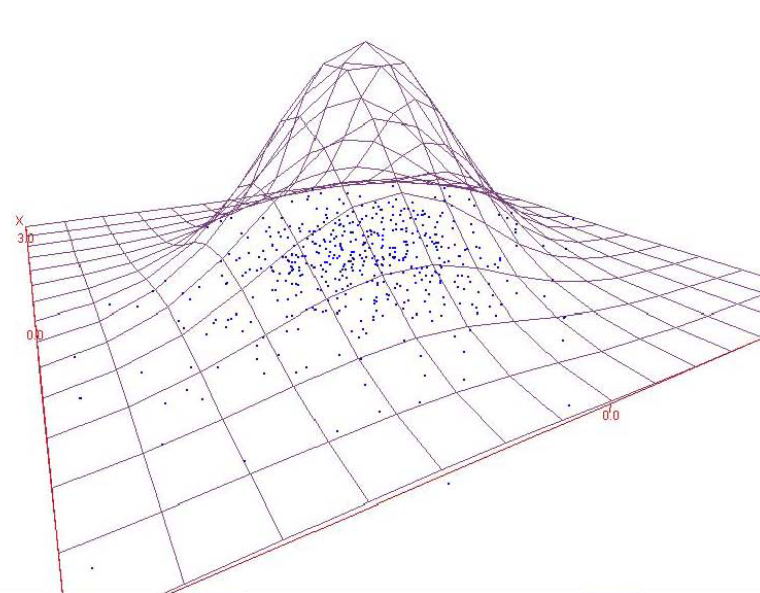
\includegraphics[scale=0.6]{img/NormalBivariante.png}
    \caption{Ejemplo de distribución normal bivariante}
\end{figure}

Las distribuciones marginales de una distribución Normal Bivariante son normales unidimensionales,

\[ X_1\thicksim N(\mu_1,\sigma_1^2) \quad \text{y} \quad X_2\thicksim N(\mu_2,\sigma_2^2) \]

donde la correlación $\rho$ controla el grado de dependencia lineal entre ellas.

\newpage

\begin{figure}[htbp]
    \center
    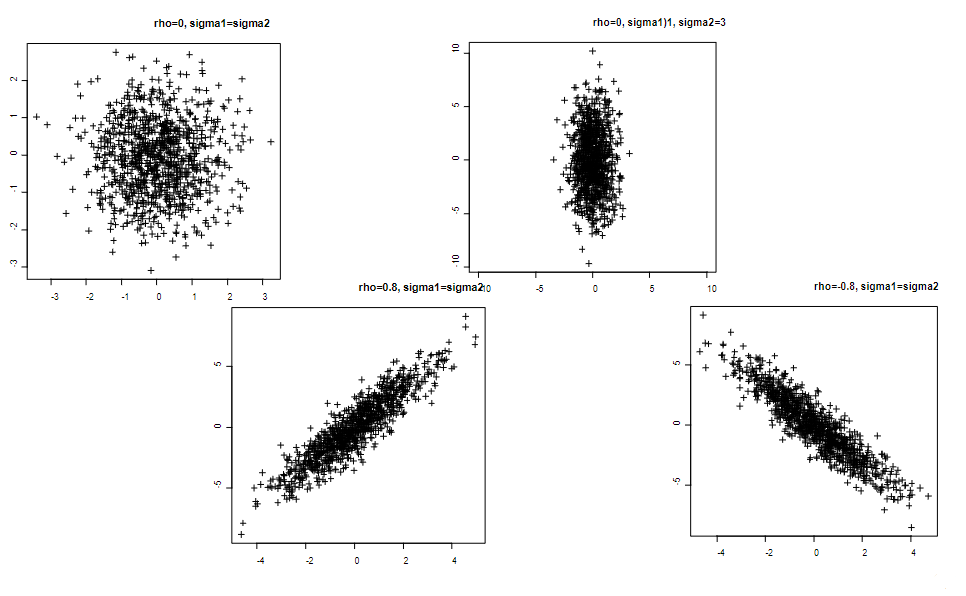
\includegraphics[scale=0.5]{img/GraficosNormalBivariable.png}
\caption{Ejemplo de distribución normal bivariante.}
\end{figure}

Las distribuciones normales bivariantes tienen las siguientes \textbf{propiedades}:
Dado $(X_1,X_2)$ un vector aleatorio normal con vector de medidas $(\mu_1,\mu_2)$ y matriz de varianzas y covarianzas $\Sigma$,
\begin{itemize}
    \item Si $\rho = 0$ entonces $X_1$ e $X_2$ son independientes
    \item Dados $a_1,a_2,a_3 \in \mathbb{R}$, $a_1X_1 + a_2X_2 + a_3$ es normal
    \item $X_1 \bigg{/} X_2 = x_2$ es normal y $X_2 \bigg{/} X_1 = x_1$ es normal
    \item Sea $A \in \mathcal{M}_{2\times2}$, $X$ vector aleatorio de dimensión 2, $X\thicksim N(\mu_X, \Sigma_X)$ entonces \\ $Y=AX\thicksim N(\mu_Y, \Sigma_Y)$ donde $\mu_Y = A\mu_X$ y $\Sigma_Y = A\Sigma_XA^t$
\end{itemize}

Dado $(X, Y)$ un vector aleatorio normal con medidas $(\mu_X, \mu_Y)$ y matriz de varianzas y covarianzas $\Sigma$

\[ Y \bigg{/} X = x \thicksim N(\mu_2 + \rho(\frac{\sigma_2}{\sigma_1})(x-\mu_1), \sigma_2^2(1-\rho^2)) \]


\section{La Esperanza Condicionada como v.a.}


Al hablar de distribuciones condicionadas, tiene sentido plantearse cómo se incorpora a la esperanza de una variable información sobre el comportamiento de otra
o vector aleatorio asociado a ella. Por simplificar trataremos el caso bivariante. \\
Supongamos que $(X,Y)$ es un vector aleatorio bidimensional. La esperanza de la variable $Y$ es una caracteristica propia de la distribución de $Y$, en principio, $P_Y$.
Si conocemos que $X = x$, el modelo asociado a $Y$ pasará a estar dado por la distribución condicionada $P_{Y/X = x}$. 

\newpage

Al valor esperado de $Y$ en este modelo se le llama esperanza de $Y$ condicionada por $X=x$ y se denota

\[ E\left( Y \bigg{/} X = x \right) \]

Recordando lo estudiado sobre las distribuciones condicionadas, es fácil darse cuenta que, en el caso discreto, la forma de calcular la esperanza condicionada
está dada por la siguiente expresión:

\[ E\left( Y \bigg{/} X = x \right) = \sum_yyP\left(Y=y\bigg{/X=x}\right) = \sum_yy\frac{p(x,y)}{p_X(x)} \]

mientras que en el aso continuo la regla de cálculo para la esperanza condicionada está dada por la siguiente expresión

\[ E\left( Y \bigg{/} X = x \right) = \int yf_{Y/X=x}(y)dy = \int y\frac{f(x,y)}{f_X(x)}dy \]

Sea $(X,Y)$ vector aleatorio. La función $\phi(x) \equiv E\left( Y \bigg{/} X = x \right)$ está bien definida en el conjunto de posibles valores de $X$ y, por tanto,
tiene sentido calcular $\phi(X)$. A esta variable aleatoria se le suele denotar como

\[ E\left( Y \bigg{/} X \right) \]

y habitualmente nos referimos a ella como ``esperanza de $Y$ ''. //
$\phi(X)$ es una nueva variable aleatoria de la que se puede calcular su distribución, esperanza, varianza, etc. Por ejemplo, en el caso discreto, teniendo en cuenta
la expresión correspondiente para $E\left( Y \bigg{/} X = x \right)$,

\[ E(\phi(X)) = \sum_x \left( \sum_y y\frac{p(x,y)}{p_X(x)} \right) p_X(x) = \sum_{x,y}yp(x,y) = E(Y) \]

La esperanza condicionada tiene las siguientes \textbf{propiedades}:
\begin{itemize}
    \item Si $a,b \in \mathbf{R}$ entonces
        \[ E\left( aY_1 \bigg{/} X \right) = aE\left( Y_1 \bigg{/} X \right) + bE\left( Y_2 \bigg{/} X \right) \]
    \item $E\left( E\left( Y \bigg{/} \right) \right) = E(Y)$
    \item Para cualquier función $g$
        \[ E\left( g(X)Y \bigg{/} X \right) = g(X)E\left( Y \bigg{/} X \right) \]
\end{itemize}

\newpage

\subsection{Curva de regresión de \textit{Y} sobre \textit{X}}

Sea $(X,Y)$ un vector aleatorio nos planteamos el problema de encontrar una función $f$ que minimice el valor

\[ E(Y - f(X))^2 \]

Si tomamos la notación anterior para $\phi(x)$, entonces, de la tercera propiedad de la esperanza condicionada se deduce que

\[ E(Y -f(X))^2 = E(Y - \phi(X))^2 + E(\phi(X) - f(X))^2 \]

lo que significa que el valor mínimo de $E(Y - f(X))^2$ se alcanza cuando $f = \phi$. \\
Claro que $\phi(X) = E\left( Y \bigg{/} X \right)$. Esto significa que $\phi(X)$ es la variable aleatoria función de $X$ que
mejor aproxima a $Y$ en el sentido de los mínimos cuadrados. Por esta razón, nos referimos en ocasiones a $\phi(X)$ como la
\textit{curva de regresión de $Y$ sobre $X$}. \\

\subsection{Recta de regresión de \textit{Y} sobre \textit{X}}

Sea $(X,Y)$ un vector aleatorio nos planteamos el problema de encontrar $a,b \in \mathbb{R}$ que minimicen el valor

\[ E(Y - aX - b)^2 \]

Se puede ver que este error, como función de $b$ se minimiza cuando $b = E(Y) - aE(X)$. Entonces la función a minimizar es

\[ Var(Y - aX) = Var(Y) + a^2Var(X) - 2aCov(X,Y) \]

y el mínimo se alcanza en $a = \frac{Cov(X,Y)}{Var(X)} = \rho_{X,Y}\frac{\sigma_Y}{\sigma_X}$. Por lo tanto la función a minimizar será

\[ E(Y) + \rho_{X,Y}\frac{\sigma_Y}{\sigma_X}(X - E(X)) \]

que es la variable aletoria función lineal de $X$ que mejor representa a $Y$ en el sentido del error cuadrático. A esta variable
se la llama \textit{rectra de regresión de $Y$ sobre $X$}.

\subsection{Ejemplos}

Ejemplos \textbf{discretos}:
\begin{itemize}
    \item Vector multinomial. Las condicionadas son vinomiales y la curva de regresión es una recta
    \item Cálculos a partir de una tabla cruzada
\end{itemize}
Ejemplos \textbf{continuos}:
\begin{itemize}
    \item Vector Normal. Las condicionadas son normales y la curva de regresión es una recta.
    \item Cálculos a partir de $f(x,y)$
\end{itemize}

\subsection{La varianza condicionada como v.a.}

Sea $(X,Y)$ un vector aleatorio, definimos la v.a. en función de $X$:

\[ Var\left( Y \bigg{/} X \right) = E\left( \left( Y - E \left( Y \bigg{/} X \right) \right)^2 \bigg{/} X \right)\]

tambien podemos calcularla como:

\[ Var\left( Y \bigg{/} X \right) = E\left( Y^2 \bigg{/} X \right) - \left( E\left( Y \bigg{/} X \right) \right)^2 \]

ademas se verifica la siguiente igualdad:

\[ Var(Y) = E\left( Var\left( Y \bigg{/} X \right) \right) + Var\left( E\left( Y \bigg{/} X \right) \right) \]


\section{Distribuciones asociadas a un vector ordenado}


Sean $X_1, X_2, \dots, X_n$ v.a. cuando las ordenamos las denotamos por

\[ X_{(1)}, X_{(2)}, \dots, X_{(n)} \]

El vector $(X_{(1)}, X_{(2)}, \dots, X_{(n)})$ es un estadístico $n$-dimensional puesto que es función de la muestra, aunque en este caso el estadístico
no reduce la dimensión de ella. Este vector recibe el nombre de \textbf{estadístico ordenado}. \\
A su coordenada $X_{(i)}$ la llamaremos \textbf{estadístico ordenado $i$-esimo}. \\

La \textbf{distribución conjunta} del estadístico ordenado en el caso continuo: \\
Sean $X_1, X_2, \dots, X_n$ v.a.i.i.d. con distribución $F$ continua y sea $f$ su función de densidad, la función de densidad que define la distribución $n$-dimensional
del vector $T = (X_{(1)}, X_{(2)}, \dots, X_{(n)})$ es el siguiente producto

\[ f_T=(x_1, x_2, \dots, x_n) = n!f(x_1)f(x_2)\dotsb f(x_n) \qquad \text{si} \quad x_1 < x_2 < \dots < x_n \]

\subsection{Distribución del máximo}

Sean $X_1, X_2, \dots, X_n$ v.a.i.i.d. con distribución $F$, la función de distribución de $X_{(n)}$ es

\[ F_{X_{(n)}}(x)=F(x)^n \]

y su función de densidad de $X_{(n)}$ es

\[ f_{X_{(n)}}(x)=nf(x)F(x)^{n-1} \]

\newpage

\subsection{Distribución del mínimo}

Sean $X_1, X_2, \dots, X_n$ v.a.i.i.d. con distribución $F$, la función de distribución de $X_{(1)}$ es

\[ F_{X_{(1)}}(x)=1 - (1 - F(x))^n \]

y su función de densidad de $X_{(1)}$ es

\[ f_{X_{(1)}}(x)=nf(x)(1 - F(x))^{n-1} \]

% Versión examen
% \section{Aplicaciones a v.a. independientes igualmente distribuidas (m.a.s)}


% \newpage

% ------------------------------------------------------------------------------
% Reference and Cited Works
% ------------------------------------------------------------------------------

\begin{thebibliography}{9}
    \bibitem{article}
    Pilar Rodríguez de Tío, \\ \textit{Vectores aleatorios y distribuciones multivariantes}. \\ Universidad de Valladolid, 2023.
    \bibitem{article}
    Pilar Rodríguez de Tío, \\ \textit{Distribuciones asociadas a variables independientes igualmente distribuidas}. \\ Universidad de Valladolid, 2023.
\end{thebibliography}

% ------------------------------------------------------------------------------

\end{document}
